% SIAM Article Template
\documentclass[review,onefignum,onetabnum]{siamart190516}
\usepackage{amssymb}
\usepackage{float}
\usepackage[ruled,vlined]{algorithm2e}
% Information that is shared between the article and the supplement
% (title and author information, macros, packages, etc.) goes into
% ex_shared.tex. If there is no supplement, this file can be included
% directly.

% SIAM Shared Information Template
% This is information that is shared between the main document and any
% supplement. If no supplement is required, then this information can
% be included directly in the main document.


% Packages and macros go here
\usepackage{lipsum}
\usepackage{amsfonts}
\usepackage{graphicx}
\usepackage{epstopdf}
\usepackage{algorithmic}
\ifpdf
  \DeclareGraphicsExtensions{.eps,.pdf,.png,.jpg}
\else
  \DeclareGraphicsExtensions{.eps}
\fi

% Add a serial/Oxford comma by default.
\newcommand{\creflastconjunction}{, and~}

% Used for creating new theorem and remark environments
\newsiamremark{remark}{Remark}
\newsiamremark{hypothesis}{Hypothesis}
\crefname{hypothesis}{Hypothesis}{Hypotheses}
\newsiamthm{claim}{Claim}

% Sets running headers as well as PDF title and authors
\headers{An Example Article}{D. Doe, P. T. Frank, and J. E. Smith}

% Title. If the supplement option is on, then "Supplementary Material"
% is automatically inserted before the title.
\title{An Example Article\thanks{Submitted to the editors DATE.
\funding{This work was funded by the Fog Research Institute under contract no.~FRI-454.}}}

% Authors: full names plus addresses.
\author{Dianne Doe\thanks{Imagination Corp., Chicago, IL 
  (\email{ddoe@imag.com}, \url{http://www.imag.com/\string~ddoe/}).}
\and Paul T. Frank\thanks{Department of Applied Mathematics, Fictional University, Boise, ID 
  (\email{ptfrank@fictional.edu}, \email{jesmith@fictional.edu}).}
\and Jane E. Smith\footnotemark[3]}

\usepackage{amsopn}
\DeclareMathOperator{\diag}{diag}


%%% Local Variables: 
%%% mode:latex
%%% TeX-master: "ex_article"
%%% End: 


\title{Optimal Sensor Placement for Learning Initial Conditions of Differential Equations}

\author{J. E. Smith}

% The next statement enables references to information in the
% supplement. See the xr-hyperref package for details.

\externaldocument{ex_supplement}

% FundRef data to be entered by SIAM
%<funding-group specific-use="FundRef">
%<award-group>
%<funding-source>
%<named-content content-type="funder-name"> 
%</named-content> 
%<named-content content-type="funder-identifier"> 
%</named-content>
%</funding-source>
%<award-id> </award-id>
%</award-group>
%</funding-group>

\begin{document}

\maketitle

% REQUIRED
\begin{abstract}
  In this paper, we are interested in learning initial conditions of differential equations. We formulate the problem in a machine learning context and only require sparse data observation. We then propose fast algorithms for strategically choosing those sparse observations. 
\end{abstract}

% REQUIRED
\begin{keywords}
  example, \LaTeX
\end{keywords}

% REQUIRED
\begin{AMS}
\end{AMS}

\section{Introduction}

Often, when we want to infer the initial condition of a system of differential equations from data gathered in the real world, we don't have complete access to all the spatial and temporal data. For example, when we want to infer the initial temperature profile of a 1-D rod governed by the heat equation, $ {\partial t} X(t,x) = k{\Delta X (t,x)} $, we cannot know the temperature reading for every discretized point during the entire observation period. What is likely in reality is that we may have several temperature sensors at our disposal. We can record temperature reading at a finite number of points on this 1-D rod and then infer the initial temperature profile of this 1-D rod. 

This real world setting presents us with several challenges. First, given a finite number of sensors, how should we strategically place those sensors so that we can learn the initial condition accurately? Second, once the data is gathered, how should we solve the inverse problem given the sparsely observed data? Third, when a discretization scheme for a differential equation presents large matrices or when then differential equations involve high dimensions, computation can be costly. How should we solve the optimal sensor problem efficiently? 

We will answer each of those questions in the paper and provide the necessary convergence proof along the way. We will start by formulating the mathematical inverse problem in the context of machine learning. In section 2, the related work section, we will present several ideas ranging from learning differential equations from data, physics-based machine learning, and optimal actuator placement problem. In section 3, we will present the necessary background on control theory and implicitly constrained optimization problems. 


\subsection{Problem formulation -- learning differential equations}
 In modern machine learning, often the role of automatically discovering the behavior of a system and predicting its future state is done by a deep neural network. However, a human being can hardly decipher a deep neural network as supposed to differential equations. Differential equations can often provide some insight into a phenomenon, such as employing Newton's second law for describing the trajectory of a ball or Maxwell's equations for explaining electromagnetism. We want to leverage ideas from machine learning and describes one particular method of discovering differential equations from observed data. 

We formulate the mathematical problem of learning differential equations from observed data as the following:
\begin{equation}
\begin{aligned}
&\text{minimize}
&&\lVert \mathcal{C}X -Y_{obs} \rVert^2+\alpha \lVert z \rVert^2\\
& \text{subject to}
&& \mathcal{L}(X ,z) = 0
\end{aligned}
\end{equation}
The objective function we want to minimize in this machine learning setting is given by $\lVert \mathcal{C}X -Y_{obs} \rVert^2+\alpha \lVert z \rVert^2$. In particular, $Y_{obs}$ is the observed data, $X$ is the true state of the system. However, often, we cannot have direct access to the true state of the system, and this is modeled by the $\mathcal{C}$ operator. For instance, if the system in inquiry is governed by Schrodinger's equation, then we cannot directly measure the wave function. The actual measured data is obtained by applying some observation operator to the true state of the system, and we use $\mathcal{C}$ to denote this observation operator. $z$ is some parameter of the system that we don't know yet but want to learn, and $\alpha$ is a regularization hyper parameter. We want to fit the observed data to the model, which is why we want to minimize $\lVert \mathcal{C}X -Y_{obs} \rVert^2$. At the same time, we want to avoid over fitting, and this is achieved by the regularization term, $\alpha \lVert z \rVert^2$. 

This objective function is subjected to a constraint equation, $\mathcal{L}(X ,z) = 0$. In the setting of learning differential equations, the constraint equation takes the form of differential equations. If the part of the differential equations we want to learn are scalar parameters, such as the diffusivity parameter of a heat equation, then $z$ can be the diffusivity parameter. In this heat equation setting, if the problem is 1-D, then the constraint function can be $ {\partial t} X(t,x) = z{\Delta X (t,x)} $, with $z$  being the diffusivity parameter. 


\section{Related work}

People have developed methods to incorporate apriori knowledge for better learning the structure of the observed data. One such method is described by Xiaowei Jia et al in \cite{xiaowei}. In their work, they want to model temperature profiles for a lake based on Long-Short Term Memory (LSTM) neural networks. Instead of directly applying the LSTM to fit the observed data, they incorporate energy conservation law  in the LSTM. They do so by adding a physics based penalty term. The new loss function in their paper is now:
\begin{equation}
\mathcal{L} = \mathcal{L}_{LSTM}+\lambda_{EC}\mathcal{L}_{EC}
\end{equation}
$\mathcal{L}_{EC}$ is a term that ensures the total energy in the lake is consistent with energy conservation. $\mathcal{L}_{LSTM}$ is comparing the difference between observed data and LSTM predicted data. $\lambda_{EC}$ is a hyper-parameter that balance the loss the standard LSTM loss and energy conservation loss. Though this method can allow apriori mechanistic knowledge to be encoded into the machine learning process, the LSTM cannot easily provide new understanding of the observed data. 

Another approach of incorporating apriori mechanistic knowledge into the data discovering process is introduced by Raissi and et al in \cite{raissi}. In their work, they place a Gaussian process prior on solutions of differential equations. In this framework, unknown scalar parameters of differential equations are then turned into hyper parameters of kernel functions employed in the Gaussian process. Thus, by minimizing the negative log marginal likelihood function, they are able to learn those scalar parameters of the differential equations from observed data. This approach offers a lot of interpretability and can bypass the need for solving differential equations either analytically or numerically. However, this approach cannot learn more complex parts of unknown differential equations, such as initial condition or boundary condition. 

We believe the mathematical problem formulated in equation 1.1 can offer the level of interpretability of differential equations yet flexible enough to learn representation of spatial and temporal functions. 

Another area of related work we want to present is on control theory. In a paper published by Tyler Summers et al \cite{summers}, they investigated how to choose a finite number of actuators for controlling an electrical grid. In this paper, they presented several scalar objective functions that one should optimize for controlling. They investigated the structure of those scalar objective functions and found them to be either modular or submodular set functions. However, in the area of control theory, little work has been work for optimal sensor placement for learning conditions of a dynamical system. 

\section{Background}
\subsection{Linear time-invariant dynamical system}

We begin with the state space form of a linear time-invariant (LTI) dynamical system:
\begin{equation}
\begin{aligned}
M\dot{x}(t) = Ax(t)+Bu(t)\\
y(t) = Cx(t)+Du(t)+\epsilon\\
\end{aligned}
\end{equation}
The state vector is x(t) $\in \mathbb{R}^{N}$. The input or control is modeled as u(t) $\in \mathbb{R}^{M}$. The output is  y(t) $\in \mathbb{R}^{P}$. In the context of learning differential equations,  M $\in \mathbb{R}^{N*N}$ is usually obtained through the discretization process. The dynamics matrix is A $\in \mathbb{R}^{N*N}$ . The input matrix is B $\in \mathbb{R}^{N*M}$. The sensor matrix is C $\in \mathbb{R}^{P*N}$. The feedthrough matrix is D $\in \mathbb{R}^{P*M}$. 

We can then rewrite the above system of equations as:
\begin{gather}
 \begin{bmatrix} y(0)\\...\\y(t-1) \end{bmatrix}
 = Ox(0) + T \begin{bmatrix} u(0)\\...\\u(t-1) \end{bmatrix}
 + \begin{bmatrix} \epsilon\\...\\\epsilon \end{bmatrix}
\end{gather}
where

\begin{gather}
 O = \begin{bmatrix} C\\CM^{-1}A\\...\\C(M^{-1}A)^{t-1} \end{bmatrix}
\end{gather}

\begin{gather}
T = \begin{bmatrix} 
 D & 0 & ... \\
 CB & D & 0 & ...\\
 ...\\
 C(M^{-1}A)^{t-2}B & C(M^{-1}A)^{t-3}B & ... & CB & D
 \end{bmatrix}
\end{gather}

To obtain an estimation of $X(0)$ with the presence of noise, we the invoke the least square method. The solution for this least square method is
\begin{equation}
    x_{ls}(0) = x(0)+O^{\dagger}\begin{bmatrix} \epsilon\\...\\\epsilon \end{bmatrix}
\end{equation}
or
\begin{equation}
    x_{ls}(0) = O^{\dagger}\bigg(\begin{bmatrix} y(0)\\...\\y(t-1) \end{bmatrix} - T \begin{bmatrix} u(0)\\...\\u(t-1) \end{bmatrix}\bigg)
\end{equation}
and $O^{\dagger}$ is the Moore-Penrose pseudo-inverse, $O^{\dagger} = (O^{T}O)^{-1}O$. To make the least square method as robust as possible to noise, we want the smallest eigenvalue of the $O$ matrix to be as large as possible. 

\subsection{Observability gramian}
We need to introduce the observability gramian. The observability gramian for a LTI dynamical system described in equation 3.1 can be obtained by solving the generalized lyapunov equation. The matrix Q appearing in the generalized lyapunov equation is the observability gramian. 

\begin{equation}
    A^{T}QM + MQA+C^{T}C = 0
\end{equation}

Generally one might be interested in computing the observability gramian because if Q is full rank, than the standard control theory tells us that one can solve the initial condition exactly by inverting the O matrix in equation 3.2. 
We are interested in the observability gramian because one can express $x_{ls}(0)$ in the following way:

\begin{equation}
    x_{ls}(0) = \bigg(\sum_{\tau - 0}^{t-1} (M^{-1}A^{T})^{\tau}C^{T}C(M^{-1}A^{\tau})\bigg)^{-1}
    \sum_{\tau = 0}^{t-1}(M^{-1}A^{T})^{\tau}C^{T}\Tilde{y}(\tau)
\end{equation}
where $\Tilde{y} = y-h*u$, where h is impulse response and * is convolution.  
Now, 
\begin{equation}
    \sum_{\tau - 0}^{t-1} (M^{-1}A^{T})^{\tau}C^{T}C(M^{-1}A^{\tau})
\end{equation}
is the observability gramian

\subsection{Properties of log det of observability gramian} First, we will introduce the concept of submodularity and monotone increasing. Then, we will state that the log determinant of the observability gramian is a submodular  and monotone increasing set function. Lastly, we will argue a way of solving this optimization problem. 

Sensor placement problems can be formulated as set function optimization problems. For a given finite set $V = \{1,2,...,M\}$, a set function $f:2^{V} \to R$ assigns a real number to each subset of V. In the problem of optimal sensor placements for learning initial conditions, the elements of V represent potential sensor locations. 

\begin{definition}
Submodularity. A set function $f:2^{V} \to R$ is called submodular if for all subsets A 
$\subseteq$ B $\subseteq$ V and all elements s $\notin$ B, it holds that 
\begin{equation}
    f(A\cup \{s\})-f(A) \geqslant f(B\cup\{s\})-f(B)
\end{equation}
\end{definition}
Intuitively, submodularity means we get diminishing returns. We can understand equation 3.8 as stating that adding an element to a smaller set gives a larger return than adding an element to a larger set. 

\begin{definition}
A set function $f:2^{V} \to R$ is called monotone increasing if for all subsets A,B $\subseteq$ V it holds that
\begin{equation}
    A \subseteq B \to f(a) \leqslant f(b)
\end{equation}
\end{definition}

Intuitively, this means adding an element to a set always gives a positive return.

Tyler Summers et al in \cite{summers} proofed that the log determinant of controllability gramian is submodular and monotone increasing. Because controllability gramians and observability gramians are duals of each other, the log determinant of observability gramian is also submodular and monotone increasing. 

Because the log determinant of observability gramian is submodular and monotone increasing, once can solve such an optimization problem by the greedy algorithm. 
\begin{theorem}\cite{greedy}
Let $f^{*}$ be the true optimal solution of a set function optimization problem. Let $f(S_{greedy})$ be the solution of the set function optimization problem obtained from applying the greedy algorithm. If f is submodular and monotone increasing, then 
\begin{equation}
    \frac{f^{*}-f(S_{greedy})}{f^{*}-f(\emptyset)} \leqslant
    \bigg(\frac{k-1}{k}\bigg)^{k} \leqslant
    \frac{1}{e} \approx 0.37
\end{equation}
\end{theorem}
In the above equation, k denotes the size of the set. The bound guarantee is the best for any polynomial time algorithm, assuming $P \ne NP$. Also, one should note that this is a worst-case bound. Often, the greedy algorithm performs better than this bound. 

\subsection{SVD update} Here, we want to provide the background of how to update a singular value decomposition. Let X $\in \mathbb{R}^{p*q}$ have rank r and economy SVD $USV^{T} = X$ with S $\in \mathbb{R}^{r*r}$. Let A $\in \mathbb{R}^{p*c}$ and B $\in \mathbb{R}^{q*c}$ be two matrices of rank c. We want to know the SVD of the sum of $X+AB^{T}$
\[ X+AB^{T}=  
\left( \begin{array}{cc}
U & A \\
\end{array} \right)
%
\left( \begin{array}{cc}
S & 0 \\
0 & I
\end{array} \right)
%
\left( \begin{array}{cc}
V & B \\
\end{array} \right)^T
\]
To compute this update efficiently, we need to first perform two QR decompositions, $PR_{A} = (I-UU^{T})A$ and $QR_{B} = (I-VV^{T})B$. The idea is that P will than be an orthogonal basis for the component of A that is orthogonal to U. Similarly, Q will be an orthogonal basis for the component of B that is orthogonal to V. We can now rewrite $[U~A]$ and $[V ~ B]^{T}$ as
\[ 
\left( \begin{array}{cc}
U & A \\
\end{array} \right) 
= 
\left( \begin{array}{cc}
U & P \\
\end{array} \right)
%
\left( \begin{array}{cc}
I & U^{T}A \\
0 & R_{A}
\end{array} \right)
\]

\[ 
\left( \begin{array}{cc}
V & B \\
\end{array} \right)^T
= 
\left( \begin{array}{cc}
I & V^{T}B \\
0 & R_{B}
\end{array} \right)^T
%
\left( \begin{array}{cc}
V & Q\\
\end{array} \right)^T
\]
So, we can rewrite $X+AB^T$ as $[U ~ P]K[V ~ Q]^T$. 
\[ K =  
\left( \begin{array}{cc}
I & U^{T}A \\
0 & R_{A}
\end{array} \right)
%
\left( \begin{array}{cc}
S & 0 \\
0 & I
\end{array} \right)
%
\left( \begin{array}{cc}
I & V^{T}B \\
0 & R_{B}
\end{array} \right)^T
\]

Usually this K matrix is small in size, highly structured, and sparse. We can complete the SVD update step by performing an SVD decomposition on this K matrix, $K = U'S'V'^{T}$. Finally, 
\begin{equation}
    X+AB^T = ([U ~ P]U')S'([V ~ Q]V')^{T}
\end{equation}
For more details on SVD update, we recommend \cite{svd-update}.

\subsection{Solving constrained optimization}Recall the constrained optimization problem. 
\begin{equation}
\begin{aligned}
&\text{minimize}
&&\lVert \mathcal{C}X -Y_{obs} \rVert^2+\alpha \lVert z \rVert^2\\
& \text{subject to}
&& \mathcal{L}(X ,z) = 0
\end{aligned}
\end{equation}
We begin to solve this constrained minimization problem by first rewriting the problem in the form of an unconstrained minimization problem. Notice the constraint equation, $\mathcal{L}(X ,z) = 0$. This equation tells us that for every z, we can solve the constraint equation and obtain an corresponding X. Let's call this mapping from z to X as $\psi: \psi(z) = X$. So, $\lVert \mathcal{C}X -Y_{obs} \rVert^2+\alpha \lVert z \rVert^2$ becomes $\lVert \mathcal{C}\phi(z) -Y_{obs} \rVert^2+\alpha \lVert z \rVert^2$. Notice that the objective function is now just a function of the unknown z, which we can solve by Newton-Conjugate Gradient. The Newton equation we want to solve is $\nabla^2 f(z) d = -\nabla f(z)$, where $f(z) = \lVert \mathcal{C}\phi(z) - Y_{obs} \rVert^2+\alpha \lVert z \rVert^2$ and d is step size. So, the task now is computing the gradient and applying the Hessian to a vector. 
\begin{algorithm}[H]
%\SetAlgoLined
1. Given z, solve ${L}(X ,z) = 0$. Denote the solution by $X(z)$ \\
2. Solve $\lambda$ in the adjoint equation: $\mathcal{L}_{X}(X(z) ,z)^{*}\lambda = 
    -f_{X}(X(z) ,z)$ \\
3. Compute the gradient: $\nabla f(z) = f_{z}(X(z),z)+
    \mathcal{L}_{z}(X(z) ,z)^{*}\lambda$
 \caption{Gradient Computation Using Adjoints}
\end{algorithm}
The star operator in the adjoint equation means the adjoint operation. In this context, since the discretized differential equations usually result in matrices, the adjoint operation usually means the adjoint of matrices. The subscript in the above algorithm means the variable we are taking derivative with respect to. We will also use this notation in the Hessian-Times-Vector algorithm. 

\begin{algorithm}[H]
%\SetAlgoLined
 Given v, the vector in the Hessian-Times-Vector Computation\\
 \\
1. Given z, solve ${L}(X ,z) = 0$. Denote the solution by $X(z)$. (If not done already.)\\
2. Solve $\lambda$ in the adjoint equation: $\mathcal{L}_{X}(X(z) ,z)^{*}\lambda = 
    -f_{X}(X(z) ,z)$. (If not done already.) \\
3. Solve s in the sensitivity equation: $\mathcal{L}_{X}(X(z) ,z)s = 
    \mathcal{L}_{z}(X(z) ,z)v$\\
4. Solve p in the adjoint sensitivity equation: $\mathcal{L}_{X}(X(z) ,z)^{*}p = 
    LG_{XX}(X(z) ,z)s-
    LG_{Xz}(X(z) ,z)v$\\
5. Compute the result of applying Hessian to a vector: $\nabla^2 f(z) v = \mathcal{L}_{z}(X(z),z)^{*}p-
    LG_{zX}(X(z) ,z)s+
    LG_{zz}(X(z) ,z)v$
 \caption{Hessian-Times-Vector Computation}\\
\end{algorithm}

LG means Lagrangian in the above algorithm. It takes the form of $f(X,z)+k\mathcal{L}(X ,z)$, or objective function plus a scalar multiple of constraint equation. For more details of solving constrained optimization problems, one is encouraged to look at this reference \cite{Heinkenschloss08numericalsolution}

% The outline is not required, but we show an example here.
% The paper is organized as follows. Our main results are in
% \cref{sec:main}, our new algorithm is in \cref{sec:alg}, experimental
% results are in \cref{sec:experiments}, and the conclusions follow in
% \cref{sec:conclusions}.

\section{Main results}
\label{sec:main}

We start this section by first stating a method of computing the observability gramian analytically. 

\subsection{A suitable objective function}
A common strategy for choosing optimal sensor placement in control theory is by optimizing an objective function from scalarizing the observability gramian. Common scalarization includes the trace of the observability gramian, the trace of the inverse of the observability gramian, and the log determinant of the observability gramian. Among those scalarization schemes, we need to find one that is particular suited for learning initial conditions. Recall 

\begin{equation}
    x_{ls}(0) = \bigg(\sum_{\tau - 0}^{t-1} (M^{-1}A^{T})^{\tau}C^{T}C(M^{-1}A^{\tau})\bigg)^{-1}
    \sum_{\tau = 0}^{t-1}(M^{-1}A^{T})^{\tau}C^{T}\Tilde{y}(\tau)
\end{equation}
and 
\begin{equation}
    Observability ~ Gramian (OG) = \sum_{\tau - 0}^{t-1} (M^{-1}A^{T})^{\tau}C^{T}C(M^{-1}A^{\tau})
\end{equation}

Therefore, in order for the initial condition to be as robust as possible to noise, we want the smallest eigenvalue of the observability gramian to be as large as possible. So the objective function for determining optimal sensor placement should maximize the smallest eigenvalue of the observability gramian. Tyler Summers et al in \cite{summers} randomly generated 10,000 discrete stable dynamics system. For each of the randomly generated system, they apply the greedy algorithm to select 7 actuators from a set of possible 25 for different scalarized controllability gramians. Then, they computed the eigenvalues of the controllability gramian and averaged over those 10,000 samples. The result is shown below:

\begin{figure}[H]
    \centering
    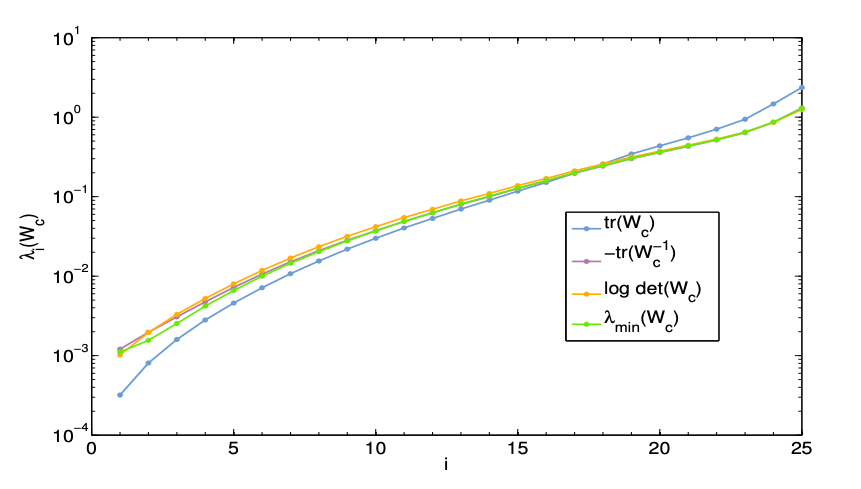
\includegraphics[width=8cm]{objective_experiment.png}
    \caption{Numerical experiment from Tyler Summers}
    %\label{fig:galaxy}
\end{figure}

From the graph, it's clear that Trace is not the optimal scalarization procedure for the problem of learning initial conditions. Of the other three scalarization schemes, it appears the effect on the smallest eigenvalue of the controllability gramian is the same. So, the second criteria of choosing a better scalarization procedure is considering how efficient it is to carry out the computation and how amenable the scalarization procedure is to numerical low rank approximation. So, we decided to use the log determinant scalarization schemes. 


\subsection{Computing observability gramian} We start with the M matrix from the LTI dynamical system in equation 3.1, which is a symmetric positive definite matrix with size n by n. Usually, this M matrix is the mass matrix after discretizing a differential equation, and the size of the M matrix corresponds to the number of spatial discretization points. After obtaining this M matrix, we perform an eigenvalue decomposition. $M = UKU^{T}$. Then, we define two matrices $\hat{U}$ and $\hat{A}$. $\hat{U} = Uinv(K^{1/2})$ and $\hat{A} = \hat{U}^TA\hat{U}$. Then, we diagonalize the matrix $\hat{A}$, and have $\hat{A} = VLV^{T}$. Lastly, we obtain a matrix W, $W = \hat{U}V = Uinv(K^{1/2})V$. In doing those four steps, we have essentially performed a change of basis such that $W^{T}MW = I$ and $W^TAW = L$, where A is the dynamics matrix in the LTI dynamical system. We are now able to write down an analytical expression for the observability gramian, 
\begin{equation}
Observability ~ Gramian (OG) = W\int_{0}^{\infty} exp(Lt)W^TC^TMCWexp(Lt) dt ~ W^{T}\\
\end{equation}
Recall the C matrix is the observation operator in the LTI dynamical system. For a more detailed treatment of those steps and the integral form of the observability gramian, we recommend this reference \cite{analytical-og}. 



\subsection{Low rank structure of the observability gramian} We have empirically observed that there is a numerically low rank structure within the observability gramian. The numerically low rank structure comes from that the L matrix described in section 4.1 is diagonal and its diagonal entries decay rather quickly. For example, suppose the LTI dynamical system is obtained by applying the finite element discretization scheme on the 1-D heat equation. Suppose the spatial dimension extends from [0,1]. Let's denote $x_{i}$ by $x_{i} = ih$ with h = $\frac{1}{n+1}$ for i = 0,1,...n+1 the mesh along the spatial dimension. Let the basis function be 

\[
  \phi(x) =
  \begin{cases}
                                   x & \text{if $x \in [0,1)$} \\
                                   2-x & \text{if $ x \in [1,2]$} \\
  0 & \text{otherwise}
  \end{cases}
\]
translated and scaled to interpolate at the mesh vertices $x_{i}$. That is, $\phi_{i}(x) = \phi(\frac{x-x_{i-1}}{x_{i}-x_{i-1}})$ We associate with the mesh vertices $x_{0}$ and $x_{n+1}$ the one-sided hat functions. For illustration, we discretize the 1-D heat equation with 98 interior mesh points, or 100 mesh points in total. We observe the diagonal entries of the L matrix exhibits the following pattern. 

\begin{figure}[H]
    \centering
    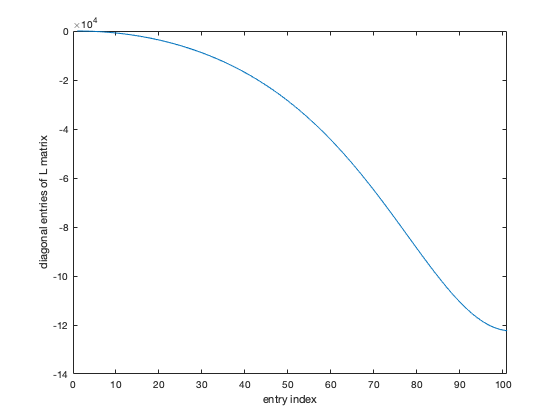
\includegraphics[width=6cm]{diag of l matrix.png}
    \caption{Diagonal entries of L matrix}
    %\label{fig:galaxy}
\end{figure}
We are able to explicitly compute the integral that appears in the observability gramian expression, 
\begin{equation}
\int_{0}^{\infty} exp(Lt)W^TC^TMCWexp(Lt) dt 
\end{equation}
Let's denote $W^TC^TMCW$, or everything that is sandwiched between the two $exp(Lt)$, as Middle. Then, the ijth entry of the matrix given by the above integral is 
\begin{equation}
Integral_{ij} = Middle_{ij}\int_{0}^{\infty} exp[(L_{ii}+L_{jj})t] ~ dt
\end{equation}
\begin{equation}
Integral_{ij} = Middle_{ij}\frac{-1}{L_{ii}+L_{jj}}
\end{equation}

To illustrate the low rank structure, we randomly place $10\%$, $30\%$, and $50\%$ of all possible sensors. For this heat equation example, because the basis functions are hat functions, this corresponds to randomly setting 10, 30, and 50 entries of the diagonal of an all zero matrix to 1s. After explicitly computing the integral, we are able to visualize those three matrices. We can plot the log of the absolute value of entries of those matrices. 


\begin{figure}[!htb]
\minipage{0.32\textwidth}
  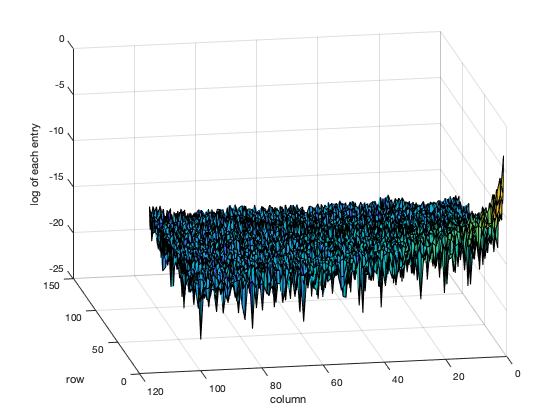
\includegraphics[width=\linewidth]{10_percent.png}
  \caption{$10\%$ random observation}\label{fig:awesome_image1}
\endminipage\hfill
\minipage{0.32\textwidth}
  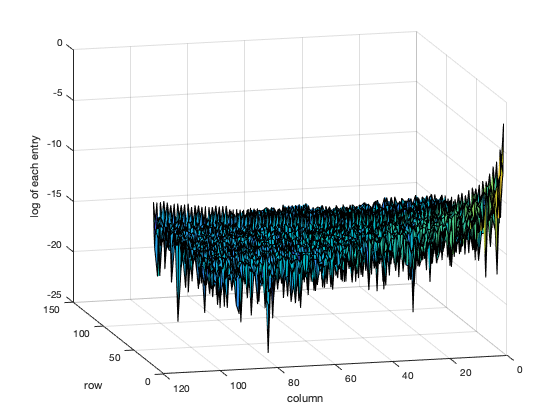
\includegraphics[width=\linewidth]{30_percent.png}
  \caption{$30\%$ random observation}\label{fig:awesome_image2}
\endminipage\hfill
\minipage{0.32\textwidth}%
  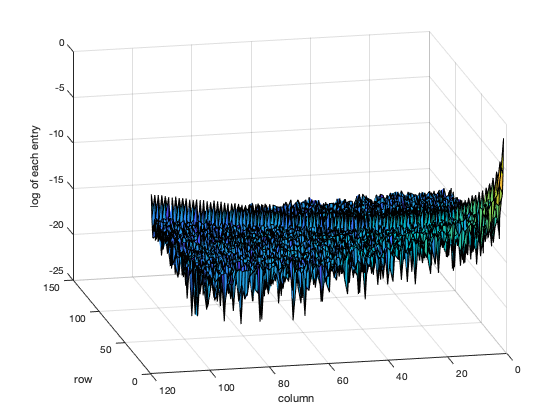
\includegraphics[width=\linewidth]{50_percent.png}
  \caption{$50\%$ random observation}\label{fig:awesome_image3}
\endminipage
\end{figure}

We noticed that the magnitude of the entries near the (0,0) location far exceeds that of other entries. We sorted the diagonal entries of the L matrix on a descending order, and therefore the entries of the integral near the (0,0) location have large magnitude. Furthermore, the rate at which the magnitude of the entries decreases as we move away from the (0,0) location is also fast. Both the magnitude and the decreasing speed allows us to numerically approximate the entire observability gramian by only entries near the (0,0) location. 

\subsection{Additive relation of the observability gramian} There is an additive relation of the observability gramian. Namely, when we add a new sensor to an existing set of sensors, we can write the observability gramian of the combined set as the addition of the observability gramian of the existing set and the observability gramian of the new sensor. For the observation operator, C, we will use $C_{old}$ to denote the effect of the existing set of sensors, and $C_{new}$ to denote the effect of a new sensor. 

\begin{equation}
\begin{aligned}
& & OG = W\int_{0}^{\infty} exp(Lt)W^T(C_{old}+C_{new})^TM(C_{old}+C_{new})Wexp(Lt) dt ~ W^{T}\\
\end{aligned}
\end{equation}

\begin{equation}
\begin{aligned}
& OG = W\int_{0}^{\infty} exp(Lt)W^TC_{old}^TMC_{old}Wexp(Lt) dt ~ W^{T}\\
& +W\int_{0}^{\infty} exp(Lt)W^T(C_{new}^TMC_{new}+C_{new}^TMC_{old}+C_{old}^TMC_{new})Wexp(Lt) dt ~ W^{T}\\
\end{aligned}
\end{equation}

Because the observability gramian is a symmetric positive definite matrix, the singular values are identical to eigenvalues. Therefore, when we compute the log determinant of the observability gramian, we can first compute the singular values. Suppose we are in an iteration of the greedy algorithm and we know the singular value decomposition of the observability gramian of the existing set of sensors. 
\begin{equation}
    U_{old}S_{old}V_{old} = W\int_{0}^{\infty} exp(Lt)W^TC_{old}^TMC_{old}Wexp(Lt) dt ~ W^{T}
\end{equation}
To compute the effect of a new sensor on the observability gramian, and therefore on the objective function, we really need to just compute the following integral, which we denote as $Integral_{update}$
\begin{equation}
\begin{aligned}
&&Integral_{update} = \int_{0}^{\infty} exp(Lt)W^T(C_{new}^TMC_{new}+\\
&&C_{new}^TMC_{old}+C_{old}^TMC_{new})Wexp(Lt) dt. 
\end{aligned}
\end{equation}
Then, 
\[ OG =  \left( \begin{array}{cc}
U_{old} & W \\
\end{array} \right)
%
\left( \begin{array}{cc}
S_{old} & 0 \\
0 & Integral_{update}
\end{array} \right)
%
\left( \begin{array}{cc}
V_{old} & W \\
\end{array} \right)^T
\]

So, the idea is that instead of solving the observability gramian from scratch each time we add a new sensor, we just need to compute the $Integral_{update}$ term and do a SVD update. Usually, computing $Integral_{update}$ is not extremely costly, as usually there are some structure for the $C_{new}$ and $C_{old}$ operators to be exploited. 

\subsection{Fast algorithms} We can now exploit both the additive relation and the low rank structure, especially in the context of the greedy algorithm. Because from one iteration to the next iteration of the greedy algorithm, only one new sensor is added.
So, we can use the SVD update structure described before. The greedy algorithm and the additive relation go hand in hand together for a fast algorithm. We can further accelerate the algorithm for optimal sensor placement in large systems by taking advantage of the numerical low rank structure of the $Integral_{update}$ term. 

\subsubsection{Using top eigenvalues}
Naturally, for a large system, the objective is the log determinant of the top H eigenvalues. If we want to get a rather accurate approximation of the top H eigenvalues, we want to compute more than just a H by H matrix starting with the (0,0) entry for the $Integral_{update}$ term. We want to compute more than just the first H by H entries. We introduce a parameter $n_{integral}$ to denote the number of entries of the integral we want to compute explicitly starting from the (0,0) entry. For a LTI dynamical system with n spatial discretization points, we propose the following algorithm for efficiently selecting $n_{sensor}$ sensors. 


\begin{algorithm}[H]
\SetAlgoLined
 Given $n_{integral}$, $n_{sensor}$\\
1. Set $selected\_obs$ as an empty set. \\
2. $M = UKU^{T}$, $\hat{U} = Uinv(K^{1/2})$, $\hat{A} = \hat{U}^{T}A\hat{U}$, $\hat{A} = VLV^{T}$, $W = \hat{U}V $\\
3. Select the first $n_{integral}$ number of columns of W and denote this as $W_{truncated}$\\
4. Initialize $U_{old}$ as a zero matrix of size n by $n_{integral}$. Fill the main diagonal of $U_{old}$ with 1s. Initialize $S_{old}$ as a zero matrix of size $n_{integral}$ by $n_{integral}$. Initialize $V_{old}$ exactly as $U_{old}$.\\

\For{i = 0,1,2,...$n_{sensor}$}{\\
1. Do a QR decomposition, $PR_{A} = (I-U_{old}U_{old}^{T})W_{truncated}$ \\
2. Form $K_{left}$ as 
\left( \begin{array}{cc}
I & U_{old}^{T}W_{truncated} \\
0 & R_{A}
\end{array} \right)\\


3. Do a QR decomposition, $QR_{B} = (I-V_{old}V_{old}^{T})W_{truncated}$\\
4. Form $K_{right}$ as 
\left( \begin{array}{cc}
I & V_{old}^{T}W_{truncated} \\
0 & R_{B}
\end{array} \right)\\

\For{j = 0,1,2,...n}{
\If{j not in set $selected\_obs$}{
1. Compute the first $n_{integral}$ by $n_{integral}$ entries of $Integral_{update}$ and denote the result as $I_{low ~ rank}$.\\
2. Compute K. K = $K_{left}$
\left( \begin{array}{cc}
S_{old} & 0 \\
0 & I_{low ~ rank}
\end{array} \right)
$K_{right}^{T}$\\
3. Compute a SVD decomposition of K. $U'S'V'^{T} = K$\\
4. Select the top H singular values of S' and compute the objective. \\
5. Record the objective function value for this sensor location. \\
}
}
5. Find the new sensor location. Denote this location as $j_{new sensor}$\\
6. Compute the first $n_{integral}$ by $n_{integral}$ entries of $Integral_{update}$ based on $j_{new sensor}$. Denote the result as $I_{low ~ rank}$.\\
7. Compute K. K = $K_{left}$
\left( \begin{array}{cc}
S_{old} & 0 \\
0 & I_{low ~ rank}
\end{array} \right)
$K_{right}^{T}$\\
8. Compute a SVD decomposition of K. $U'S'V'^{T} = K$\\
9. Set $U_{old}$ as the first $n_{integral}$ columns of $[U_{old} P]U'$. \\
10. Set $S_{old}$ as the first the first $n_{integral}$ by $n_{integral}$ entries of $S'$\\
11. Set $V_{old}$ as the first  $n_{integral}$ columns of $[V_{old} Q]V'$. \\
12. Add $j_{new sensor}$ to the set $selected\_obs$
}
 \caption{Fast Algorithm for Log Determinant of Top H Eigenvalues}
\end{algorithm}

For the two QR decompositions, both $(I-U_{old}U_{old}^{T})W_{truncated}$ and its counterpart $(I-V_{old}V_{old}^{T})W_{truncated}$ have size n by $n_{integral}$. So, the time complexity for the QR decomposition is $\mathcal{O}(nn_{integral}^2)$. For the inner for loop, usually there are some structures for computing $W^T(C_{new}^TMC_{new}+C_{new}^TMC_{old}+C_{old}^TMC_{new})W$. So the cost of computing $I_{low ~ rank}$ is $\mathcal{O}(n_{integral}^2)$. The cost of forming K in the inner loop is $\mathcal{O}((2n_{integral})^3)$. The cost of SVD decomposition is $\mathcal{O}((2n_{integral})^3)$. After finding a new optimal sensor location, the cost of forming K again is $\mathcal{O}((2n_{integral})^3)$, and then we have to perform one more SVD decomposition, which costs $\mathcal{O}((2n_{integral})^3)$. Since we only need the first $n_{integral}$ columns of  $[U_{old} P]U'$, the cost of update $U_{old}$ is  $\mathcal{O}(n2n_{integral}n_{integral})$

So, the most computation expensive part of the inner for loop is forming the K matrix and computing its SVD. In general, we have to repeat this process n times for a new sensor iteration. So, the total time complexity of finding one more new sensor for this algorithm is bounded above by $\mathcal{O}(nn_{integral}^2+n((2n_{integral})^3))$, where the first term comes from the QR decompositive and the second term comes from the inner loop of the algorithm. One should note that if the objective is the log determinant of top H eigenvalues, then $n_{integral} \ll n$. 

\subsubsection{Predefined subspace}
Sometimes, we may not be interested in using the top H eigenvalues of the observability gramian as the objective function. For instance, we may want to reproduce the learned initial conditions. Sometimes we are restricted by the types of equipment we have at our disposal and can only reproduce certain kinds of initial conditions. For instances like this and other similar cases, we want to project the observability gramian into a predefined subspace and use the log determinant of the observability gramian projected into this predefined subspace as the objective function for determining optimal sensor location. 

Suppose G is an orthonormal basis for a g-dimensional subspace of $R^{n}$. We want to use $logdet(G^{T}~OG~G)$ as the objective function, where OG is shorthand for observability gramian. There is a nice connection between using $logdet(G^{T}~OG~G)$ as the objective function and using log determinant of the top H eigenvalues of the observability gramian as the objective function. Suppose we can diagonalize the observability gramian in the G basis, $OG = GDG^{T}$. Now, we select the top H eigenvectors and form a n by H matrix by stacking the selected eigenvectors column by column. Let's denote this matrix as $G_{H}$. Now, the general expression $logdet(G^{T}~OG~G)$ becomes $logdet(G_{H}^{T}~GDG^{T}~G_{H})$. Because the orthogonality property of G, $logdet(G_{H}^{T}~GDG^{T}~G_{H})$ is computing the log determinant of the top H eigenvalues of the observability gramian.

\begin{algorithm}[H]
\SetAlgoLined
 Given a matrix G, the rank of matrix g, a scalar parameter $n_{integral}$, total sensor number $n_{sensor}$\\
1. Set $selected\_obs$ as an empty set. \\
2. $M = UKU^{T}$, $\hat{U} = Uinv(K^{1/2})$, $\hat{A} = \hat{U}^{T}A\hat{U}$, $\hat{A} = VLV^{T}$, $W = \hat{U}V $\\
3. Compute $W_{projected}' = G^{T}W$. Then, select the first $n_{integral}$ number of columns of $W_{projected}'$ and denote this as $W_{projected}$\\
4. Create a zero matrix Z of size g by g and initialize $U_{old}S_{old}V_{old}' = SVD(Z)$

\For{i = 0,1,2,...$n_{sensor}$}{\\
1. Do a QR decomposition, $PR_{A} = (I-U_{old}U_{old}^{T})W_{projected}$ \\
2. Form $K_{left}$ as 
\left( \begin{array}{cc}
I & U_{old}^{T}W_{truncated} \\
0 & R_{A}
\end{array} \right)\\


3. Do a QR decomposition, $QR_{B} = (I-V_{old}V_{old}^{T})W_{projected}$\\
4. Form $K_{right}$ as 
\left( \begin{array}{cc}
I & V_{old}^{T}W_{truncated} \\
0 & R_{B}
\end{array} \right)\\

\For{j = 0,1,2,...n}{\\
\If{j not in set $selected\_obs$}{
1. Compute the first $n_{integral}$ by $n_{integral}$ entries of $Integral_{update}$ and denote the result as $I_{low ~ rank}$.\\
2. Compute K. K = $K_{left}$
\left( \begin{array}{cc}
S_{old} & 0 \\
0 & I_{low ~ rank}
\end{array} \right)
$K_{right}$\\
3. Compute a SVD decomposition of K. $U'S'V'^{T} = K$\\
4. Select the top g singular values of S' and compute the objective. \\
5. Record the objective function value for this sensor location. \\
}
}
5. Find the new sensor location. Denote this location as $j_{new ~ sensor}$\\
6. Compute the first $n_{integral}$ by $n_{integral}$ entries of $Integral_{update}$ based on $j_{new~sensor}$. Denote the result as $I_{low ~ rank}$.\\
7. Compute K. K = $K_{left}$
\left( \begin{array}{cc}
S_{old} & 0 \\
0 & I_{low ~ rank}
\end{array} \right)
$K_{right}$\\
8. Compute a SVD decomposition of K. $U'S'V'^{T} = K$\\
9. Set $U_{old}$ as the first $n_{integral}$ columns of $[U_{old} P]U'$. \\
10. Set $S_{old}$ as the first the first $n_{integral}$ by $n_{integral}$ entries of $S'$\\
11. Set $V_{old}$ as the first  $n_{integral}$ columns of $[V_{old} Q]V'$. \\
12. Add $j_{new sensor}$ to the set $selected\_obs$
}

 \caption{Fast Algorithm for $logdet(G^{T}~OG~G)$}
\end{algorithm}

For the two QR decompositions, both $(I-U_{old}U_{old}^{T})W_{projected}$ and its counterpart $(I-V_{old}V_{old}^{T})W_{projected}$ have size g by $n_{integral}$. So, the time complexity for the QR decomposition is $\mathcal{O}(gn_{integral}^2)$. For the inner for loop, usually there are some structures for computing $W^T(C_{new}^TMC_{new}+C_{new}^TMC_{old}+C_{old}^TMC_{new})W$. So the cost of computing $I_{low ~ rank}$ is $\mathcal{O}(n_{integral}^2)$. The cost of forming K in the inner loop is $\mathcal{O}(2g(g+n_{integral})2g)$. The cost of SVD decomposition is $\mathcal{O}((2g)^3)$. After finding a new optimal sensor location, the cost of forming K again is $\mathcal{O}(2g(g+n_{integral})2g)$, and then we have to perform one more SVD decomposition, which costs $\mathcal{O}((2g)^3)$. Since we only need the first $n_{integral}$ columns of  $[U_{old} P]U'$, the cost of update $U_{old}$ is  $\mathcal{O}(2g^{3})$

So, the most computation expensive part of the inner for loop is forming the K matrix and computing its SVD. In general, we have to repeat this process n times for a new sensor iteration. So, the total time complexity of finding one more new sensor for this algorithm is bounded above by $\mathcal{O}(gn_{integral}^2+n(4g^{2}(g+n_{integral})))$, where the first term comes from the QR decompositive and the second term comes from the inner loop of the algorithm. Typically, g is a very small number, and $n_{integral} \ll n$. 

\section{Experimental results}
\subsection{Heat equation} We are interested in learning the initial condition of the 1-D heat equation, and the problem can be formulated as the following:

\begin{equation}
\begin{aligned}
& \underset{X_{0}}{\text{minimize}}
& & \frac{1}{2} \int_{0}^{T} \int_{D} (CX(t,x)-Y_{obs}(t,x))^2 dx dt + \frac{\alpha}{2} \int_{D} X_{0}(x)^2 dx\\
& \text{subject to}
& & {\partial t} X(t,x) = k{\Delta X (t,x)} \\
&&& \frac{\partial X(t,x)}{\partial n} = \gamma(U(t,x)-X(t,x)) \\
&&& X(0,x) = X_{0}(x)
\end{aligned}
\end{equation}

There are three equations acing as the constraint to this constrained minimization problem. The 1-D heat equation is , ${\partial t} X(t,x) = k{\Delta X (t,x)}$, there the scalar k is the diffusivity of the medium. This differential equation is paired with a Robin boundary condition, $\frac{\partial X(t,x)}{\partial n} = \gamma(U(t,x)-X(t,x))$, where U describes the temperature at the two ends of this 1-D rod, or boundary control, and $\gamma$ describe the diffusivity at the ends of the 1-D rod. The initial condition for this 1-D heat equation is $X(0,x) = X_{0}(x)$. 

To arrive at the weak form, we multiply both sides of the PDE by a sufficiently regular test function, $V(x)$, integrate by parts, and we arrive at:
\begin{center}
\begin{equation}
\begin{split}
    \int_D {\partial t} X(t,x) V(x) dx + \int_D K <\nabla X(t,x),\nabla V(x)> dx
    + \int_{\partial D} k \gamma X(t,x)V(x) dx \\
    = - \int_{\partial D} k \gamma U(t,x)V(x) dx 
\end{split}
\end{equation}
\end{center}

Suppose the spatial dimension extends from [0,1]. Let's denote $x_{i}$ by $x_{i} = ih$ with h = $\frac{1}{n+1}$ for i = 0,1,...n+1 the mesh along the spatial dimension. Let the basis function be 

\[
  \phi(x) =
  \begin{cases}
                                   x & \text{if $x \in [0,1)$} \\
                                   2-x & \text{if $ x \in [1,2]$} \\
  0 & \text{otherwise}
  \end{cases}
\]
translated and scaled to interpolate at the mesh vertices $x_{i}$. That is, $\phi_{i}(x) = \phi(\frac{x-x_{i-1}}{x_{i}-x_{i-1}})$ We associate with the mesh vertices $x_{0}$ and $x_{n+1}$ the one-sided hat functions, $\psi$. We approximate the heat equation solution and the boundary control as


\begin{equation}
\begin{aligned}
    X &= \sum_{i = 0}^{n+1} x_{i}\phi_{i}           &  U &= \sum_{i = 0}^{1} u_{i}\psi_{i}
\end{aligned}
\end{equation}

Substituting the approximation expression into the weak form, and setting $V(x) = \phi_{u}$, we have 

\begin{equation}
\begin{aligned}
    &\sum_{i = 0}^{n+1} \partial_{t} x_{i} \int_{D} \phi_{i}(x) \phi_{j}(x) dx = \\
    &\sum_{i = 0}^{n+1}\bigg\{ -x_{i}\int_{D} \nabla\phi_{i}(x) \nabla\phi_{j}(x)  dx
    -x_{i} \gamma \int_{\partial_{D}} \phi_{i}(x) \phi_{j}(x)  dx \bigg\}
    + \sum_{i = 0}^{1}u_{i}\gamma\int_{\partial_{D}} \phi_{i}(x) \phi_{j}(x)  dx
\end{aligned}
\end{equation}



for j = 0,1,...,n+1. This results in the system of differential equations

\begin{equation}
    M\dot{X} = AX + BU
\end{equation}

where M $\in \mathbb{R}^{(n+2)*(n+2)}$,A $\in \mathbb{R}^{(n+2)*(n+2)}$, and B $\in \mathbb{R}^{(n+2)*(2)}$ are
\begin{equation}
    M_{ij} = \int_{D} \phi_{i}(x) \phi_{j}(x)  dx
\end{equation}

\begin{equation}
    A_{ij} = -\int_{D} \nabla\phi_{i}(x) \nabla\phi_{j}(x)  dx
    - \gamma\int_{\partial_{D}} \phi_{i}(x) \phi_{j}(x)  dx
\end{equation}
and 
\begin{equation}
    B_{ij} = \gamma\int_{\partial_{D}} \phi_{i}(x) \phi_{j}(x)  dx
\end{equation}
 
 We then approximate the time dimension of the differential equation, $M\dot{X} = AX + BU$, by the $\theta-method$. Let $0<t_{0}<t_{1}...<t_{N}<t_{N+1} = 1$ denote a partition of the time dimension spanning [0,1], where $t_{i} = i\delta t$ and $\delta t = \frac{1}{N+1}$. The $\theta-method$ results in 
 
 \begin{equation}
     (M-\theta\delta t A)x_{i+1} = (M+(1-\theta)\delta t A)x_{i} + \delta t B (\theta u_{i+1}+(1-\theta) u_{i})
 \end{equation}

After approximating the constraint differential equation, we now approximate the objective function. The approximation is
\begin{equation}
\begin{split}
& \frac{1}{2} \delta t \bigg\{  (1-\theta) (x_{0}-y_{0})^\top C^\top M C (x_{0}-y_{0})\\
&  + \sum_{i=1}^{N} (x_{i}-y_{i})^\top C^\top M C (x_{i}-y_{i}) \\
&  + \theta (x_{N+1}-y_{N+1})^\top C^\top M C (x_{N+1}-y_{N+1}) \bigg\} \\
& + \frac{\alpha}{2} u_{0}^\top M u_{0}
\end{split}
\end{equation}

After setting up the proper differential equation and the objective function in the chosen basis, we need to determine where the optimal sensor locations are. The basis functions are localized hat functions translated and scaled on [0,1], so mathematically the optimal sensor problem is represented by determining which entries on the diagonal of the C matrix are 1s and which are 0s. For this numerical experiment, we discretize the 1-D rod on [0,1] to 300 interior points, and we want to choose the optimal sensor locations for the first 40 sensors First, we are going to demonstrate the result of the fast algorithm when the objective function for choosing optimal sensor location is log det of top H eigenvalues. In general, the eigenvalues of the observability gramian decays exceedingly quickly. Here, we have plotted the eigenvalues of the observability gramian for randomly selecting $20\%$ of discretized points for this example. 

\begin{figure}[!htb]
\minipage{0.5\textwidth}
  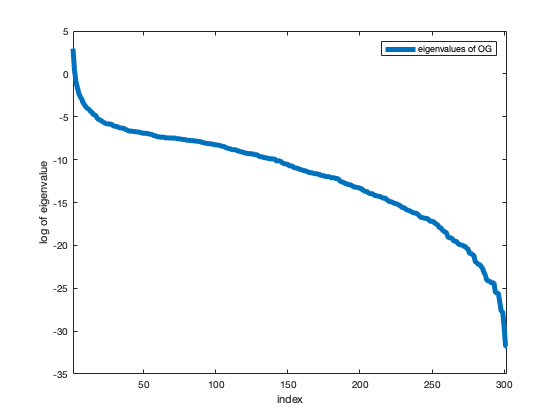
\includegraphics[width=\linewidth]{all_eig.png}
  \caption{log of all eigenvalues}\label{fig:awesome_image1}
\endminipage\hfill
\minipage{0.5\textwidth}
  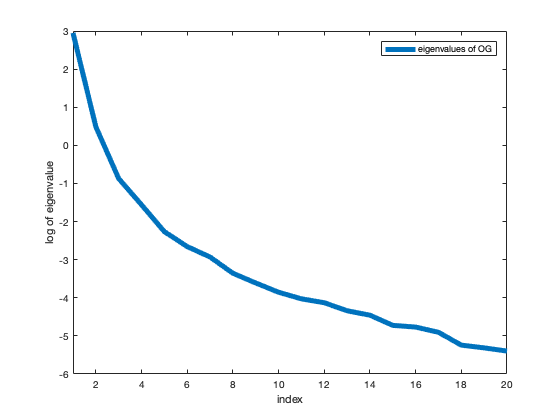
\includegraphics[width=\linewidth]{top_eig.png}
  \caption{log of top 20 eigenvalues}\label{fig:awesome_image2}
\endminipage\hfill
\end{figure}

In order for the approximation to be valid, we have selected to use the log of top 10 eigenvalues as the objective, or setting H in algorithm to be 10. We have also selected to set $n_{integral}$ to be 70. The benckmark we are comparing to is by solving the generalized lyapunov equation exactly and then compute the log det of the top 10 eigenvalues based on the exact solution. 

\begin{figure}[!htb]
\minipage{0.5\textwidth}
  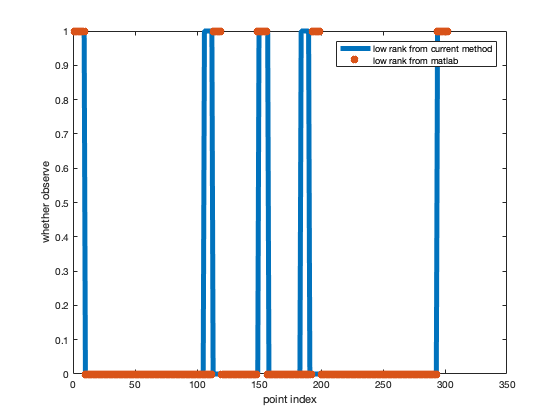
\includegraphics[width=\linewidth]{numerical_result_top_h.png}
  \caption{Objective cutoff is top 10 eigenvalues}\label{fig:awesome_image1}
\endminipage\hfill
\minipage{0.5\textwidth}
  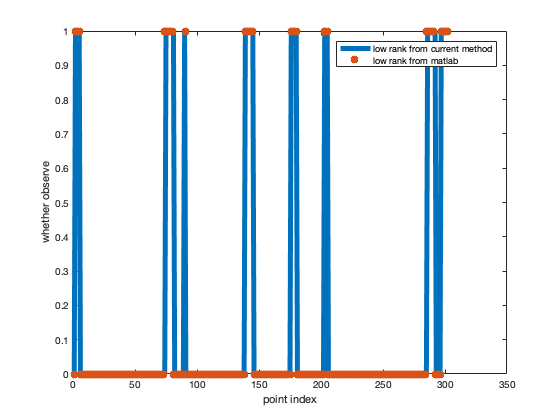
\includegraphics[width=\linewidth]{numerical_result_given_basis.png}
  \caption{Objective is based on given basis}\label{fig:awesome_image2}
\endminipage\hfill
\end{figure}

In another numerical experiment setting, we want to demonstrate the algorithm when a predefined subspace is given. Here, we randomly generated a 300 by 10 matrix with orthonormal columns, which will serve as the G matrix in algorithm 4.2. Because the orthonormal columns are not the top 10 eigenvectors of the observability gramian, we generally need to set $n_{integral}$ to be larger for the approximation to be good. Here, we are interested in the positions of the first 40 sensors. We set $n_{integral}$ to be 130 for this numerical experiment. 

Now, we want to solve the initial condition problem by leveraging the fast algorithm. We generated an initial condition and founded the minimum number of sensors needed to recover this particular initial condition. For comparison, we ask a random number generator to select the same amount of sensors but at random positions. We then compared the quality of the recovered initial condition based on those two observation scheme. In terms of the parameters of the fast algorithm, we selected 10 sensors by setting the objective as the log det of top 10 eigenvalues. 

\begin{figure}[!htb]
\minipage{0.5\textwidth}
  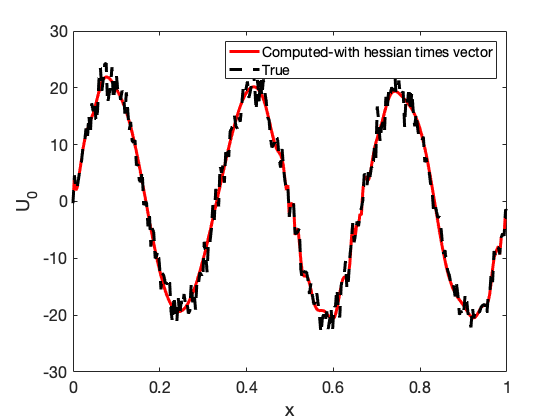
\includegraphics[width=\linewidth]{good initial condition.png}
  \caption{Carefully selected sensor placement}\label{fig:awesome_image1}
\endminipage\hfill
\minipage{0.5\textwidth}
  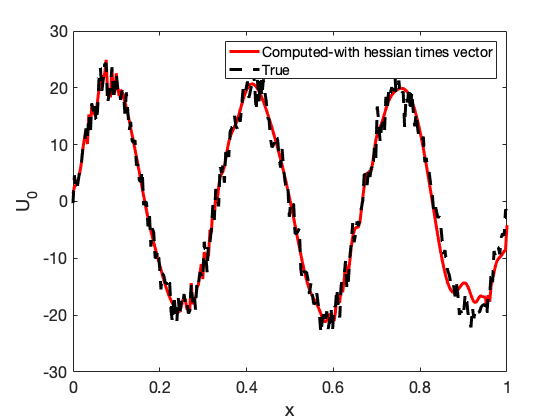
\includegraphics[width=\linewidth]{bad initial condition.png}
  \caption{Randomly selected sensor placement}\label{fig:awesome_image2}
\endminipage\hfill
\end{figure}


% With the choose basis, the explicit form of the M $\in \mathbb{R}^{(n+2)*(n+2)}$,A $\in \mathbb{R}^{(n+2)*(n+2)}$, and B $\in \mathbb{R}^{(n+2)*(2)}$ matrices are:
% \begin{gather}
%  M = h/6 \begin{bmatrix} 
%  2 & 1 \\
%  1 & 4 & 1\\
%  \ddots & \ddots & \ddots\\
%  && 1 & 4 & 1\\
%  &&& 1 & 2 
%  \end{bmatrix}
% \end{gather}

Because we are randomly selecting 10 positions out of 302 possible positions for sensor placement, sometimes the sensor placements are clustered and suboptimal. It can be seen from the right graph that maybe more sensors are needed near the right ends. However, when we are selecting sensors based on log det of observability gramian, we noticed the algorithm always places two sensors near the two ends and then place one sensor in the middle. Afterwards, the algorithm places sensors in between those points. Intuitively, this sensor placement does seem better than random placement. 






\bibliographystyle{siamplain}
\bibliography{references}
\end{document}
